\documentclass[12pt,a4paper]{article}
\usepackage[utf8]{inputenc}
\usepackage[english]{babel}
\usepackage[T1]{fontenc}
\usepackage{amsmath}
\usepackage{amsfonts}
\usepackage{amssymb}
\usepackage{makeidx}
\usepackage{graphicx}
\usepackage{kpfonts}
\usepackage[left=3cm,right=2cm,top=3cm,bottom=3cm]{geometry}
\usepackage{float}
\usepackage{adjustbox}
\usepackage{booktabs}
\usepackage{multirow}
\newcommand\x{\times}
\begin{document}
In this tests are considered 6 types of combinations:
\begin{itemize}
\item $c1$
\begin{center}
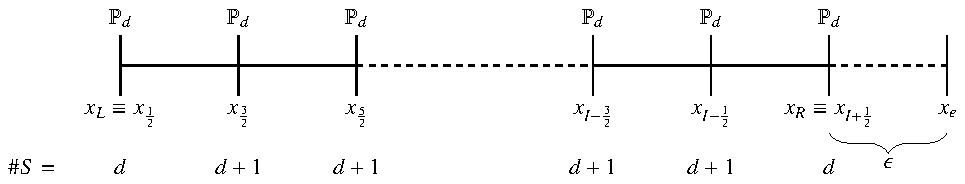
\includegraphics[width=.75\textwidth]{images/c1.pdf}
\end{center}
\item $c2$
\begin{center}
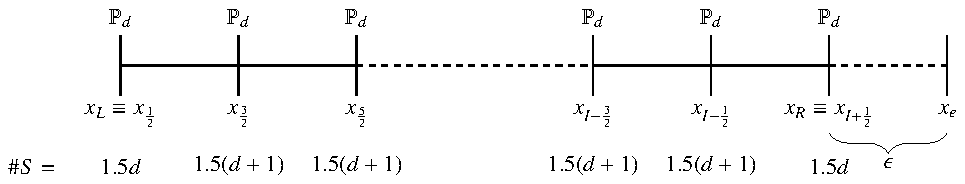
\includegraphics[width=.75\textwidth]{images/c2.pdf}
\end{center}
\item $c3$
\begin{center}
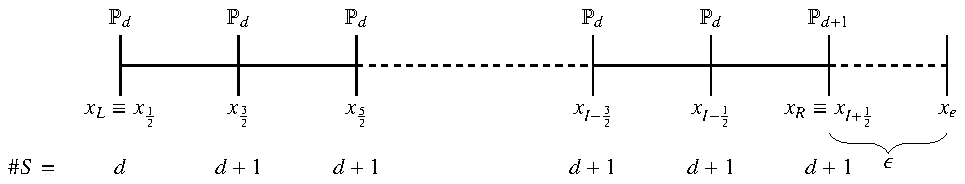
\includegraphics[width=.75\textwidth]{images/c3.pdf}
\end{center}
\item $c4$
\begin{center}
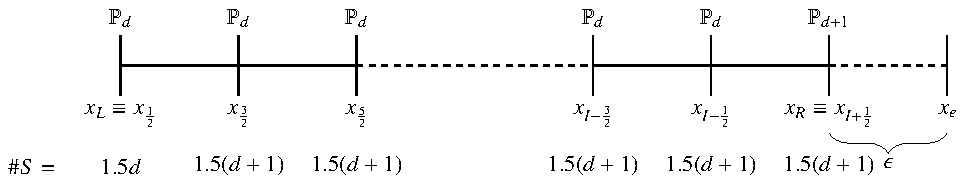
\includegraphics[width=.75\textwidth]{images/c4.pdf}
\end{center}
\item $c5$
\begin{center}
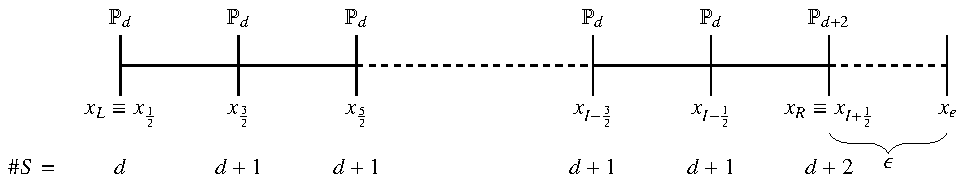
\includegraphics[width=.75\textwidth]{images/c5.pdf}
\end{center}
\item $c6$
\begin{center}
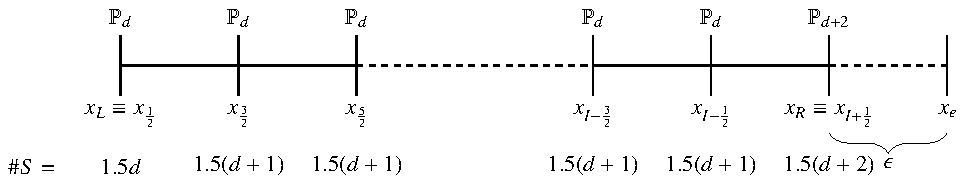
\includegraphics[width=.75\textwidth]{images/c6.pdf}
\end{center}
\end{itemize}
\pagebreak
\section*{$\epsilon=h/2$ -- uniform mesh}
\begin{table}[H]
\centering
\caption{Numerical results of pure diffusion for $\phi(x)=\exp(x)$, $\kappa(x)=1$, and $u(x)=0$ (c1).}
\begin{tabular}{@{}l c c l c c l c@{}}
\toprule
 & $I$ & cond(A) & E$_1$ & O$_1$ && E$_{\infty}$ & O$_{\infty}$\\
\midrule
\multirow{3}{*}{$\mathbb{P}_{1}$}
 & 20 & 6.48E$+$02 & 3.38E$-$02 & --- && 6.63E$-$02 & ---\\
 & 30 & 1.46E$+$03 & 2.26E$-$02 & 1.00 && 4.46E$-$02 & 0.98\\
 & 40 & 2.59E$+$03 & 1.70E$-$02 & 1.00 && 3.36E$-$02 & 0.99\\
\midrule
\multirow{3}{*}{$\mathbb{P}_{2}$}
 & 20 & 8.75E$+$02 & 1.12E$-$03 & --- && 2.13E$-$03 & ---\\
 & 30 & 1.93E$+$03 & 5.00E$-$04 & 2.00 && 9.56E$-$04 & 1.98\\
 & 40 & 3.40E$+$03 & 2.81E$-$04 & 2.00 && 5.40E$-$04 & 1.98\\
\midrule
\multirow{3}{*}{$\mathbb{P}_{3}$}
 & 20 & 1.13E$+$03 & 3.86E$-$05 & --- && 7.34E$-$05 & ---\\
 & 30 & 2.46E$+$03 & 1.14E$-$05 & 3.00 && 2.21E$-$05 & 2.96\\
 & 40 & 4.29E$+$03 & 4.82E$-$06 & 3.00 && 9.40E$-$06 & 2.97\\
\midrule
\multirow{3}{*}{$\mathbb{P}_{4}$}
 & 20 & 1.50E$+$03 & 6.55E$-$07 & --- && 1.26E$-$06 & ---\\
 & 30 & 3.16E$+$03 & 1.30E$-$07 & 3.99 && 2.55E$-$07 & 3.95\\
 & 40 & 5.40E$+$03 & 4.12E$-$08 & 4.00 && 8.14E$-$08 & 3.97\\
\midrule
\multirow{3}{*}{$\mathbb{P}_{5}$}
 & 20 & 2.47E$+$03 & 2.97E$-$08 & --- && 6.22E$-$08 & ---\\
 & 30 & 4.87E$+$03 & 4.39E$-$09 & 4.71 && 9.02E$-$09 & 4.76\\
 & 40 & 7.96E$+$03 & 1.10E$-$09 & 4.80 && 2.25E$-$09 & 4.83\\
\bottomrule
\end{tabular}
\end{table}
\begin{table}[H]
\centering
\caption{Numerical results of pure diffusion for $\phi(x)=\exp(x)$, $\kappa(x)=1$, and $u(x)=0$ (c2).}
\begin{tabular}{@{}l c c l c c l c@{}}
\toprule
 & $I$ & cond(A) & E$_1$ & O$_1$ && E$_{\infty}$ & O$_{\infty}$\\
\midrule
\multirow{3}{*}{$\mathbb{P}_{1}$}
 & 20 & 3.67E$+$02 & 3.96E$-$02 & --- && 8.19E$-$02 & ---\\
 & 30 & 8.28E$+$02 & 2.69E$-$02 & 0.96 && 5.56E$-$02 & 0.96\\
 & 40 & 1.47E$+$03 & 2.03E$-$02 & 0.97 && 4.21E$-$02 & 0.97\\
\midrule
\multirow{3}{*}{$\mathbb{P}_{2}$}
 & 20 & 5.58E$+$02 & 1.19E$-$03 & --- && 2.15E$-$03 & ---\\
 & 30 & 1.23E$+$03 & 5.19E$-$04 & 2.05 && 9.37E$-$04 & 2.05\\
 & 40 & 2.17E$+$03 & 2.90E$-$04 & 2.03 && 5.21E$-$04 & 2.04\\
\midrule
\multirow{3}{*}{$\mathbb{P}_{3}$}
 & 20 & 6.38E$+$02 & 1.23E$-$04 & --- && 2.34E$-$04 & ---\\
 & 30 & 1.41E$+$03 & 3.72E$-$05 & 2.96 && 7.17E$-$05 & 2.92\\
 & 40 & 2.47E$+$03 & 1.58E$-$05 & 2.97 && 3.08E$-$05 & 2.94\\
\midrule
\multirow{3}{*}{$\mathbb{P}_{4}$}
 & 20 & 8.35E$+$02 & 4.86E$-$06 & --- && 9.50E$-$06 & ---\\
 & 30 & 1.82E$+$03 & 1.02E$-$06 & 3.86 && 2.02E$-$06 & 3.82\\
 & 40 & 3.17E$+$03 & 3.29E$-$07 & 3.91 && 6.63E$-$07 & 3.88\\
\midrule
\multirow{3}{*}{$\mathbb{P}_{5}$}
 & 20 & 8.96E$+$02 & 4.14E$-$07 & --- && 7.98E$-$07 & ---\\
 & 30 & 1.94E$+$03 & 5.71E$-$08 & 4.89 && 1.12E$-$07 & 4.85\\
 & 40 & 3.39E$+$03 & 1.39E$-$08 & 4.92 && 2.73E$-$08 & 4.89\\
\bottomrule
\end{tabular}
\end{table}
\begin{table}[H]
\centering
\caption{Numerical results of pure diffusion for $\phi(x)=\exp(x)$, $\kappa(x)=1$, and $u(x)=0$ (c3; uniform mesh; $\epsilon=\frac{h}{2}$).}
\begin{tabular}{@{}l c c c l c c l c c l c c@{}}
\toprule
 & $I$ & cond(A) & $A^{-1}\geq 0$ &  E$_{c,1}$ & O$_{c,1}$ && E$_1$ & O$_1$ && E$_{\infty}$ & O$_{\infty}$\\
\midrule
\multirow{3}{*}{$\mathbb{P}_{1}$}
 & 20 & 6.87E$+$02 & $\checkmark$ & 9.15E$-$04 & --- && 7.72E$-$04 & --- && 1.70E$-$03 & ---\\
 & 40 & 2.67E$+$03 & $\checkmark$ & 2.19E$-$04 & 2.07 && 1.94E$-$04 & 1.99 && 4.35E$-$04 & 1.97\\
 & 80 & 1.05E$+$04 & $\checkmark$ & 5.34E$-$05 & 2.03 && 4.87E$-$05 & 2.00 && 1.10E$-$04 & 1.99\\
\midrule
\multirow{3}{*}{$\mathbb{P}_{2}$}
 & 20 & 9.08E$+$02 & $\checkmark$ & 7.24E$-$05 & --- && 3.45E$-$04 & --- && 7.34E$-$04 & ---\\
 & 40 & 3.47E$+$03 & $\checkmark$ & 9.36E$-$06 & 2.95 && 9.55E$-$05 & 1.85 && 2.04E$-$04 & 1.85\\
 & 80 & 1.35E$+$04 & $\checkmark$ & 1.19E$-$06 & 2.98 && 2.50E$-$05 & 1.93 && 5.35E$-$05 & 1.93\\
\midrule
\multirow{3}{*}{$\mathbb{P}_{3}$}
 & 20 & 1.24E$+$03 & $\x$ & 4.31E$-$06 & --- && 3.26E$-$05 & --- && 6.54E$-$05 & ---\\
 & 40 & 4.55E$+$03 & $\x$ & 2.75E$-$07 & 3.97 && 4.43E$-$06 & 2.88 && 8.87E$-$06 & 2.88\\
 & 80 & 1.73E$+$04 & $\x$ & 1.74E$-$08 & 3.98 && 5.77E$-$07 & 2.94 && 1.15E$-$06 & 2.94\\
\midrule
\multirow{3}{*}{$\mathbb{P}_{4}$}
 & 20 & 1.89E$+$03 & $\x$ & 1.96E$-$07 & --- && 2.60E$-$06 & --- && 5.08E$-$06 & ---\\
 & 40 & 6.31E$+$03 & $\x$ & 6.30E$-$09 & 4.96 && 1.73E$-$07 & 3.91 && 3.41E$-$07 & 3.90\\
 & 80 & 2.23E$+$04 & $\x$ & 2.00E$-$10 & 4.98 && 1.11E$-$08 & 3.95 && 2.21E$-$08 & 3.95\\
\midrule
\multirow{3}{*}{$\mathbb{P}_{5}$}
 & 20 & 3.62E$+$03 & $\x$ & 8.64E$-$09 & --- && 1.83E$-$07 & --- && 3.62E$-$07 & ---\\
 & 40 & 1.10E$+$04 & $\x$ & 1.38E$-$10 & 5.96 && 6.22E$-$09 & 4.88 && 1.24E$-$08 & 4.87\\
 & 80 & 3.48E$+$04 & $\x$ & 2.24E$-$12 & 5.95 && 2.01E$-$10 & 4.95 && 4.01E$-$10 & 4.95\\
\bottomrule
\end{tabular}
\end{table}
\begin{table}[H]
\centering
\caption{Numerical results of pure diffusion for $\phi(x)=\exp(x)$, $\kappa(x)=1$, and $u(x)=0$ (c4; uniform mesh; $\epsilon=\frac{h}{2}$).}
\begin{tabular}{@{}l c c c l c c l c c l c c@{}}
\toprule
 & $I$ & cond(A) & $A^{-1}\geq 0$ &  E$_{c,1}$ & O$_{c,1}$ && E$_1$ & O$_1$ && E$_{\infty}$ & O$_{\infty}$\\
\midrule
\multirow{3}{*}{$\mathbb{P}_{1}$}
 & 20 & 4.66E$+$03 & $\x$ & 9.50E$-$03 & --- && 9.81E$-$01 & --- && 4.93E$+$00 & ---\\
 & 40 & 1.95E$+$07 & $\x$ & 2.41E$-$03 & 1.98 && 8.65E$+$02 & $\uparrow$ && 4.50E$+$03 & $\uparrow$\\
 & 80 & 4.34E$+$14 & $\x$ & 6.06E$-$04 & 1.99 && 4.06E$+$09 & $\uparrow$ && 1.62E$+$10 & $\uparrow$\\
\midrule
\multirow{3}{*}{$\mathbb{P}_{2}$}
 & 20 & 5.60E$+$02 & $\checkmark$ & 3.52E$-$04 & --- && 6.37E$-$04 & --- && 1.48E$-$03 & ---\\
 & 40 & 2.16E$+$03 & $\checkmark$ & 4.57E$-$05 & 2.95 && 1.88E$-$04 & 1.76 && 4.31E$-$04 & 1.77\\
 & 80 & 8.51E$+$03 & $\checkmark$ & 5.82E$-$06 & 2.97 && 5.07E$-$05 & 1.89 && 1.16E$-$04 & 1.89\\
\midrule
\multirow{3}{*}{$\mathbb{P}_{3}$}
 & 20 & 6.56E$+$02 & $\checkmark$ & 1.53E$-$05 & --- && 2.74E$-$05 & --- && 6.02E$-$05 & ---\\
 & 40 & 2.51E$+$03 & $\checkmark$ & 9.80E$-$07 & 3.97 && 4.19E$-$06 & 2.71 && 8.77E$-$06 & 2.78\\
 & 80 & 9.80E$+$03 & $\checkmark$ & 6.21E$-$08 & 3.98 && 5.77E$-$07 & 2.86 && 1.18E$-$06 & 2.90\\
\midrule
\multirow{3}{*}{$\mathbb{P}_{4}$}
 & 20 & 8.76E$+$02 & $\checkmark$ & 1.16E$-$06 & --- && 2.55E$-$06 & --- && 4.95E$-$06 & ---\\
 & 40 & 3.26E$+$03 & $\checkmark$ & 3.83E$-$08 & 4.92 && 1.76E$-$07 & 3.86 && 3.34E$-$07 & 3.89\\
 & 80 & 1.25E$+$04 & $\checkmark$ & 1.24E$-$09 & 4.95 && 1.17E$-$08 & 3.91 && 2.19E$-$08 & 3.93\\
\midrule
\multirow{3}{*}{$\mathbb{P}_{5}$}
 & 20 & 9.97E$+$02 & $\checkmark$ & 5.51E$-$08 & --- && 2.15E$-$07 & --- && 4.29E$-$07 & ---\\
 & 40 & 3.61E$+$03 & $\checkmark$ & 8.80E$-$10 & 5.97 && 7.80E$-$09 & 4.79 && 1.54E$-$08 & 4.80\\
 & 80 & 1.36E$+$04 & $\checkmark$ & 1.40E$-$11 & 5.98 && 2.62E$-$10 & 4.90 && 5.16E$-$10 & 4.90\\
\bottomrule
\end{tabular}
\end{table}
\begin{table}[H]
\centering
\caption{Numerical results of pure diffusion for $\phi(x)=\exp(x)$, $\kappa(x)=1$, and $u(x)=0$ (c5; uniform mesh; $\epsilon=\frac{h}{2}$).}
\begin{tabular}{@{}l c c c l c c l c c l c c@{}}
\toprule
 & $I$ & cond(A) & $A^{-1}\geq 0$ &  E$_{c,1}$ & O$_{c,1}$ && E$_1$ & O$_1$ && E$_{\infty}$ & O$_{\infty}$\\
\midrule
\multirow{3}{*}{$\mathbb{P}_{1}$}
 & 20 & 5.29E$+$02 & $\checkmark$ & 3.50E$-$03 & --- && 1.87E$-$02 & --- && 4.08E$-$02 & ---\\
 & 40 & 2.02E$+$03 & $\checkmark$ & 9.04E$-$04 & 1.95 && 1.01E$-$02 & 0.89 && 2.17E$-$02 & 0.91\\
 & 80 & 7.90E$+$03 & $\checkmark$ & 2.30E$-$04 & 1.97 && 5.22E$-$03 & 0.95 && 1.12E$-$02 & 0.96\\
\midrule
\multirow{3}{*}{$\mathbb{P}_{2}$}
 & 20 & 1.13E$+$03 & $\x$ & 2.90E$-$04 & --- && 3.49E$-$03 & --- && 6.63E$-$03 & ---\\
 & 40 & 3.83E$+$03 & $\x$ & 3.83E$-$05 & 2.92 && 9.14E$-$04 & 1.93 && 1.76E$-$03 & 1.92\\
 & 80 & 1.38E$+$04 & $\x$ & 4.92E$-$06 & 2.96 && 2.34E$-$04 & 1.96 && 4.52E$-$04 & 1.96\\
\midrule
\multirow{3}{*}{$\mathbb{P}_{3}$}
 & 20 & 1.94E$+$03 & $\x$ & 1.24E$-$05 & --- && 1.84E$-$04 & --- && 3.51E$-$04 & ---\\
 & 40 & 6.17E$+$03 & $\x$ & 7.91E$-$07 & 3.97 && 2.47E$-$05 & 2.89 && 4.83E$-$05 & 2.86\\
 & 80 & 2.08E$+$04 & $\x$ & 5.01E$-$08 & 3.98 && 3.21E$-$06 & 2.95 && 6.34E$-$06 & 2.93\\
\midrule
\multirow{3}{*}{$\mathbb{P}_{4}$}
 & 20 & 3.64E$+$03 & $\x$ & 1.05E$-$06 & --- && 9.23E$-$06 & --- && 1.80E$-$05 & ---\\
 & 40 & 1.08E$+$04 & $\x$ & 3.47E$-$08 & 4.92 && 6.54E$-$07 & 3.82 && 1.30E$-$06 & 3.79\\
 & 80 & 3.36E$+$04 & $\x$ & 1.12E$-$09 & 4.96 && 4.34E$-$08 & 3.91 && 8.75E$-$08 & 3.90\\
\midrule
\multirow{3}{*}{$\mathbb{P}_{5}$}
 & 20 & 6.96E$+$03 & $\x$ & 4.66E$-$08 & --- && 5.64E$-$08 & --- && 1.06E$-$07 & ---\\
 & 40 & 2.02E$+$04 & $\x$ & 7.50E$-$10 & 5.96 && 2.30E$-$09 & 4.61 && 4.58E$-$09 & 4.53\\
 & 80 & 5.96E$+$04 & $\x$ & 1.20E$-$11 & 5.97 && 9.46E$-$11 & 4.61 && 1.92E$-$10 & 4.57\\
\bottomrule
\end{tabular}
\end{table}
\begin{table}[H]
\centering
\caption{Numerical results of pure diffusion for $\phi(x)=\exp(x)$, $\kappa(x)=1$, and $u(x)=0$ (c6; uniform mesh; $\epsilon=\frac{h}{2}$).}
\begin{tabular}{@{}l c c c l c c l c c l c c@{}}
\toprule
 & $I$ & cond(A) & $A^{-1}\geq 0$ &  E$_{c,1}$ & O$_{c,1}$ && E$_1$ & O$_1$ && E$_{\infty}$ & O$_{\infty}$\\
\midrule
\multirow{3}{*}{$\mathbb{P}_{1}$}
 & 20 & 3.88E$+$02 & $\checkmark$ & 4.08E$-$03 & --- && 1.23E$-$02 & --- && 2.83E$-$02 & ---\\
 & 40 & 1.52E$+$03 & $\checkmark$ & 1.05E$-$03 & 1.96 && 6.81E$-$03 & 0.85 && 1.54E$-$02 & 0.88\\
 & 80 & 6.00E$+$03 & $\checkmark$ & 2.65E$-$04 & 1.98 && 3.59E$-$03 & 0.92 && 7.99E$-$03 & 0.94\\
\midrule
\multirow{3}{*}{$\mathbb{P}_{2}$}
 & 20 & 5.85E$+$02 & $\checkmark$ & 3.13E$-$04 & --- && 4.38E$-$04 & --- && 1.08E$-$03 & ---\\
 & 40 & 2.23E$+$03 & $\checkmark$ & 4.11E$-$05 & 2.93 && 1.15E$-$04 & 1.93 && 2.85E$-$04 & 1.92\\
 & 80 & 8.67E$+$03 & $\checkmark$ & 5.27E$-$06 & 2.96 && 2.92E$-$05 & 1.97 && 7.29E$-$05 & 1.97\\
\midrule
\multirow{3}{*}{$\mathbb{P}_{3}$}
 & 20 & 6.74E$+$02 & $\checkmark$ & 1.50E$-$05 & --- && 3.88E$-$05 & --- && 8.21E$-$05 & ---\\
 & 40 & 2.55E$+$03 & $\checkmark$ & 9.47E$-$07 & 3.98 && 5.26E$-$06 & 2.88 && 1.09E$-$05 & 2.92\\
 & 80 & 9.89E$+$03 & $\checkmark$ & 5.96E$-$08 & 3.99 && 6.84E$-$07 & 2.94 && 1.39E$-$06 & 2.96\\
\midrule
\multirow{3}{*}{$\mathbb{P}_{4}$}
 & 20 & 9.88E$+$02 & $\x$ & 1.16E$-$06 & --- && 2.65E$-$06 & --- && 5.15E$-$06 & ---\\
 & 40 & 3.51E$+$03 & $\x$ & 3.78E$-$08 & 4.93 && 1.62E$-$07 & 4.03 && 3.08E$-$07 & 4.06\\
 & 80 & 1.31E$+$04 & $\x$ & 1.21E$-$09 & 4.96 && 1.01E$-$08 & 4.00 && 1.88E$-$08 & 4.03\\
\midrule
\multirow{3}{*}{$\mathbb{P}_{5}$}
 & 20 & 1.07E$+$03 & $\x$ & 5.60E$-$08 & --- && 2.83E$-$07 & --- && 5.61E$-$07 & ---\\
 & 40 & 3.77E$+$03 & $\x$ & 8.87E$-$10 & 5.98 && 9.72E$-$09 & 4.86 && 1.92E$-$08 & 4.87\\
 & 80 & 1.40E$+$04 & $\x$ & 1.40E$-$11 & 5.99 && 3.23E$-$10 & 4.91 && 6.39E$-$10 & 4.91\\
\bottomrule
\end{tabular}
\end{table}
%%%%%
\section*{$\epsilon=h^2$ -- uniform mesh}
\begin{table}[H]
\centering
\caption{Numerical results of pure diffusion for $\phi(x)=\exp(x)$, $\kappa(x)=1$, and $u(x)=0$ (c1; uniform mesh; $\epsilon=h^2$).}
\begin{tabular}{@{}l c c c l c c l c c l c c@{}}
\toprule
 & $I$ & cond(A) & $A^{-1}\geq 0$ &  E$_{c,1}$ & O$_{c,1}$ && E$_1$ & O$_1$ && E$_{\infty}$ & O$_{\infty}$\\
\midrule
\multirow{3}{*}{$\mathbb{P}_{1}$}
 & 20 & 6.48E$+$02 & $\checkmark$ & 1.16E$-$03 & --- && 2.86E$-$03 & --- && 5.87E$-$03 & ---\\
 & 40 & 2.59E$+$03 & $\checkmark$ & 2.49E$-$04 & 2.22 && 7.15E$-$04 & 2.00 && 1.49E$-$03 & 1.98\\
 & 80 & 1.04E$+$04 & $\checkmark$ & 5.72E$-$05 & 2.12 && 1.79E$-$04 & 2.00 && 3.74E$-$04 & 1.99\\
\midrule
\multirow{3}{*}{$\mathbb{P}_{2}$}
 & 20 & 8.29E$+$02 & $\checkmark$ & 6.57E$-$05 & --- && 5.36E$-$05 & --- && 1.62E$-$04 & ---\\
 & 40 & 3.30E$+$03 & $\checkmark$ & 8.94E$-$06 & 2.88 && 2.54E$-$05 & 1.08 && 6.51E$-$05 & 1.32\\
 & 80 & 1.32E$+$04 & $\checkmark$ & 1.16E$-$06 & 2.94 && 7.85E$-$06 & 1.69 && 1.93E$-$05 & 1.75\\
\midrule
\multirow{3}{*}{$\mathbb{P}_{3}$}
 & 20 & 1.02E$+$03 & $\checkmark$ & 4.10E$-$06 & --- && 2.34E$-$06 & --- && 3.90E$-$06 & ---\\
 & 40 & 4.08E$+$03 & $\checkmark$ & 2.68E$-$07 & 3.93 && 1.43E$-$07 & 4.04 && 2.41E$-$07 & 4.02\\
 & 80 & 1.63E$+$04 & $\checkmark$ & 1.72E$-$08 & 3.97 && 8.81E$-$09 & 4.02 && 1.51E$-$08 & 4.00\\
\midrule
\multirow{3}{*}{$\mathbb{P}_{4}$}
 & 20 & 1.19E$+$03 & $\checkmark$ & 1.89E$-$07 & --- && 2.26E$-$08 & --- && 4.74E$-$08 & ---\\
 & 40 & 4.74E$+$03 & $\checkmark$ & 6.18E$-$09 & 4.94 && 1.80E$-$09 & 3.65 && 4.92E$-$09 & 3.27\\
 & 80 & 1.90E$+$04 & $\checkmark$ & 1.98E$-$10 & 4.97 && 1.47E$-$10 & 3.62 && 3.82E$-$10 & 3.69\\
\midrule
\multirow{3}{*}{$\mathbb{P}_{5}$}
 & 20 & 1.37E$+$03 & $\checkmark$ & 8.38E$-$09 & --- && 2.61E$-$09 & --- && 8.76E$-$09 & ---\\
 & 40 & 5.43E$+$03 & $\checkmark$ & 1.36E$-$10 & 5.94 && 4.68E$-$11 & 5.80 && 1.55E$-$10 & 5.82\\
 & 80 & 2.17E$+$04 & $\checkmark$ & 2.21E$-$12 & 5.95 && 1.02E$-$12 & 5.52 && 2.95E$-$12 & 5.72\\
\bottomrule
\end{tabular}
\end{table}
\begin{table}[H]
\centering
\caption{Numerical results of pure diffusion for $\phi(x)=\exp(x)$, $\kappa(x)=1$, and $u(x)=0$ (c2; uniform mesh; $\epsilon=h^2$).}
\begin{tabular}{@{}l c c c l c c l c c l c c@{}}
\toprule
 & $I$ & cond(A) & $A^{-1}\geq 0$ &  E$_{c,1}$ & O$_{c,1}$ && E$_1$ & O$_1$ && E$_{\infty}$ & O$_{\infty}$\\
\midrule
\multirow{3}{*}{$\mathbb{P}_{1}$}
 & 20 & 3.67E$+$02 & $\checkmark$ & 4.41E$-$03 & --- && 8.78E$-$03 & --- && 2.14E$-$02 & ---\\
 & 40 & 1.47E$+$03 & $\checkmark$ & 1.09E$-$03 & 2.02 && 4.10E$-$03 & 1.10 && 9.98E$-$03 & 1.10\\
 & 80 & 5.91E$+$03 & $\checkmark$ & 2.70E$-$04 & 2.01 && 1.99E$-$03 & 1.05 && 4.80E$-$03 & 1.06\\
\midrule
\multirow{3}{*}{$\mathbb{P}_{2}$}
 & 20 & 5.31E$+$02 & $\checkmark$ & 3.28E$-$04 & --- && 3.98E$-$04 & --- && 1.01E$-$03 & ---\\
 & 40 & 2.11E$+$03 & $\checkmark$ & 4.21E$-$05 & 2.96 && 1.26E$-$04 & 1.66 && 3.07E$-$04 & 1.71\\
 & 80 & 8.44E$+$03 & $\checkmark$ & 5.33E$-$06 & 2.98 && 3.48E$-$05 & 1.85 && 8.40E$-$05 & 1.87\\
\midrule
\multirow{3}{*}{$\mathbb{P}_{3}$}
 & 20 & 6.01E$+$02 & $\checkmark$ & 1.40E$-$05 & --- && 1.01E$-$05 & --- && 1.80E$-$05 & ---\\
 & 40 & 2.40E$+$03 & $\checkmark$ & 9.15E$-$07 & 3.94 && 6.54E$-$07 & 3.95 && 1.20E$-$06 & 3.90\\
 & 80 & 9.57E$+$03 & $\checkmark$ & 5.85E$-$08 & 3.97 && 4.17E$-$08 & 3.97 && 7.78E$-$08 & 3.95\\
\midrule
\multirow{3}{*}{$\mathbb{P}_{4}$}
 & 20 & 7.54E$+$02 & $\checkmark$ & 1.11E$-$06 & --- && 9.46E$-$07 & --- && 2.17E$-$06 & ---\\
 & 40 & 3.00E$+$03 & $\checkmark$ & 3.71E$-$08 & 4.91 && 6.95E$-$08 & 3.77 && 1.61E$-$07 & 3.75\\
 & 80 & 1.20E$+$04 & $\checkmark$ & 1.20E$-$09 & 4.95 && 4.62E$-$09 & 3.91 && 1.09E$-$08 & 3.89\\
\midrule
\multirow{3}{*}{$\mathbb{P}_{5}$}
 & 20 & 8.01E$+$02 & $\checkmark$ & 5.29E$-$08 & --- && 3.87E$-$08 & --- && 7.74E$-$08 & ---\\
 & 40 & 3.19E$+$03 & $\checkmark$ & 8.60E$-$10 & 5.94 && 9.67E$-$10 & 5.32 && 2.11E$-$09 & 5.20\\
 & 80 & 1.28E$+$04 & $\checkmark$ & 1.38E$-$11 & 5.96 && 2.61E$-$11 & 5.21 && 5.94E$-$11 & 5.15\\
\bottomrule
\end{tabular}
\end{table}
\begin{table}[H]
\centering
\caption{Numerical results of pure diffusion for $\phi(x)=\exp(x)$, $\kappa(x)=1$, and $u(x)=0$ (c3; uniform mesh; $\epsilon=h^2$).}
\begin{tabular}{@{}l c c c l c c l c c l c c@{}}
\toprule
 & $I$ & cond(A) & $A^{-1}\geq 0$ &  E$_{c,1}$ & O$_{c,1}$ && E$_1$ & O$_1$ && E$_{\infty}$ & O$_{\infty}$\\
\midrule
\multirow{3}{*}{$\mathbb{P}_{1}$}
 & 20 & 6.51E$+$02 & $\checkmark$ & 8.66E$-$04 & --- && 4.78E$-$04 & --- && 5.89E$-$04 & ---\\
 & 40 & 2.60E$+$03 & $\checkmark$ & 2.13E$-$04 & 2.02 && 1.31E$-$04 & 1.87 && 1.71E$-$04 & 1.79\\
 & 80 & 1.04E$+$04 & $\checkmark$ & 5.28E$-$05 & 2.02 && 3.41E$-$05 & 1.94 && 4.55E$-$05 & 1.91\\
\midrule
\multirow{3}{*}{$\mathbb{P}_{2}$}
 & 20 & 8.29E$+$02 & $\checkmark$ & 7.50E$-$05 & --- && 1.59E$-$04 & --- && 3.71E$-$04 & ---\\
 & 40 & 3.30E$+$03 & $\checkmark$ & 9.54E$-$06 & 2.98 && 3.88E$-$05 & 2.03 && 9.17E$-$05 & 2.02\\
 & 80 & 1.32E$+$04 & $\checkmark$ & 1.20E$-$06 & 2.99 && 9.54E$-$06 & 2.02 && 2.27E$-$05 & 2.02\\
\midrule
\multirow{3}{*}{$\mathbb{P}_{3}$}
 & 20 & 1.03E$+$03 & $\checkmark$ & 4.40E$-$06 & --- && 1.89E$-$06 & --- && 5.52E$-$06 & ---\\
 & 40 & 4.08E$+$03 & $\checkmark$ & 2.78E$-$07 & 3.98 && 1.24E$-$07 & 3.93 && 3.68E$-$07 & 3.91\\
 & 80 & 1.63E$+$04 & $\checkmark$ & 1.75E$-$08 & 3.99 && 7.95E$-$09 & 3.97 && 2.37E$-$08 & 3.96\\
\midrule
\multirow{3}{*}{$\mathbb{P}_{4}$}
 & 20 & 1.19E$+$03 & $\checkmark$ & 2.00E$-$07 & --- && 1.65E$-$07 & --- && 3.38E$-$07 & ---\\
 & 40 & 4.74E$+$03 & $\checkmark$ & 6.36E$-$09 & 4.97 && 3.71E$-$09 & 5.48 && 7.45E$-$09 & 5.51\\
 & 80 & 1.90E$+$04 & $\checkmark$ & 2.01E$-$10 & 4.99 && 3.61E$-$11 & 6.68 && 6.50E$-$11 & 6.84\\
\midrule
\multirow{3}{*}{$\mathbb{P}_{5}$}
 & 20 & 1.37E$+$03 & $\checkmark$ & 8.76E$-$09 & --- && 9.15E$-$09 & --- && 2.21E$-$08 & ---\\
 & 40 & 5.43E$+$03 & $\checkmark$ & 1.40E$-$10 & 5.97 && 1.51E$-$10 & 5.92 && 3.69E$-$10 & 5.91\\
 & 80 & 2.17E$+$04 & $\checkmark$ & 2.24E$-$12 & 5.96 && 2.69E$-$12 & 5.82 && 6.33E$-$12 & 5.86\\
\bottomrule
\end{tabular}
\end{table}
\begin{table}[H]
\centering
\caption{Numerical results of pure diffusion for $\phi(x)=\exp(x)$, $\kappa(x)=1$, and $u(x)=0$ (c4; uniform mesh; $\epsilon=h^2$).}
\begin{tabular}{@{}l c c c l c c l c c l c c@{}}
\toprule
 & $I$ & cond(A) & $A^{-1}\geq 0$ &  E$_{c,1}$ & O$_{c,1}$ && E$_1$ & O$_1$ && E$_{\infty}$ & O$_{\infty}$\\
\midrule
\multirow{3}{*}{$\mathbb{P}_{1}$}
 & 20 & 3.69E$+$02 & $\checkmark$ & 4.08E$-$03 & --- && 6.08E$-$03 & --- && 1.59E$-$02 & ---\\
 & 40 & 1.48E$+$03 & $\checkmark$ & 1.05E$-$03 & 1.96 && 3.39E$-$03 & 0.84 && 8.55E$-$03 & 0.89\\
 & 80 & 5.92E$+$03 & $\checkmark$ & 2.65E$-$04 & 1.98 && 1.80E$-$03 & 0.91 && 4.44E$-$03 & 0.95\\
\midrule
\multirow{3}{*}{$\mathbb{P}_{2}$}
 & 20 & 5.31E$+$02 & $\checkmark$ & 3.14E$-$04 & --- && 5.42E$-$04 & --- && 1.28E$-$03 & ---\\
 & 40 & 2.11E$+$03 & $\checkmark$ & 4.11E$-$05 & 2.93 && 1.45E$-$04 & 1.90 && 3.44E$-$04 & 1.89\\
 & 80 & 8.44E$+$03 & $\checkmark$ & 5.27E$-$06 & 2.96 && 3.73E$-$05 & 1.96 && 8.87E$-$05 & 1.95\\
\midrule
\multirow{3}{*}{$\mathbb{P}_{3}$}
 & 20 & 6.01E$+$02 & $\checkmark$ & 1.50E$-$05 & --- && 1.60E$-$06 & --- && 8.67E$-$06 & ---\\
 & 40 & 2.40E$+$03 & $\checkmark$ & 9.46E$-$07 & 3.98 && 1.02E$-$07 & 3.97 && 6.22E$-$07 & 3.80\\
 & 80 & 9.57E$+$03 & $\checkmark$ & 5.96E$-$08 & 3.99 && 6.55E$-$09 & 3.97 && 4.15E$-$08 & 3.91\\
\midrule
\multirow{3}{*}{$\mathbb{P}_{4}$}
 & 20 & 7.54E$+$02 & $\checkmark$ & 1.15E$-$06 & --- && 5.32E$-$07 & --- && 1.34E$-$06 & ---\\
 & 40 & 3.00E$+$03 & $\checkmark$ & 3.78E$-$08 & 4.93 && 5.42E$-$08 & 3.30 && 1.32E$-$07 & 3.34\\
 & 80 & 1.20E$+$04 & $\checkmark$ & 1.21E$-$09 & 4.96 && 4.12E$-$09 & 3.72 && 9.89E$-$09 & 3.74\\
\midrule
\multirow{3}{*}{$\mathbb{P}_{5}$}
 & 20 & 8.02E$+$02 & $\checkmark$ & 5.60E$-$08 & --- && 3.59E$-$09 & --- && 9.43E$-$09 & ---\\
 & 40 & 3.19E$+$03 & $\checkmark$ & 8.87E$-$10 & 5.98 && 3.18E$-$10 & 3.50 && 8.82E$-$10 & 3.42\\
 & 80 & 1.28E$+$04 & $\checkmark$ & 1.40E$-$11 & 5.99 && 1.55E$-$11 & 4.36 && 3.89E$-$11 & 4.50\\
\bottomrule
\end{tabular}
\end{table}
\begin{table}[H]
\centering
\caption{Numerical results of pure diffusion for $\phi(x)=\exp(x)$, $\kappa(x)=1$, and $u(x)=0$ (c5; uniform mesh; $\epsilon=h^2$).}
\begin{tabular}{@{}l c c c l c c l c c l c c@{}}
\toprule
 & $I$ & cond(A) & $A^{-1}\geq 0$ &  E$_{c,1}$ & O$_{c,1}$ && E$_1$ & O$_1$ && E$_{\infty}$ & O$_{\infty}$\\
\midrule
\multirow{3}{*}{$\mathbb{P}_{1}$}
 & 20 & 4.79E$+$02 & $\checkmark$ & 3.49E$-$03 & --- && 6.89E$-$03 & --- && 1.74E$-$02 & ---\\
 & 40 & 1.92E$+$03 & $\checkmark$ & 9.04E$-$04 & 1.95 && 3.63E$-$03 & 0.92 && 8.98E$-$03 & 0.95\\
 & 80 & 7.69E$+$03 & $\checkmark$ & 2.30E$-$04 & 1.97 && 1.87E$-$03 & 0.96 && 4.55E$-$03 & 0.98\\
\midrule
\multirow{3}{*}{$\mathbb{P}_{2}$}
 & 20 & 7.61E$+$02 & $\checkmark$ & 2.90E$-$04 & --- && 2.70E$-$04 & --- && 7.56E$-$04 & ---\\
 & 40 & 3.02E$+$03 & $\checkmark$ & 3.83E$-$05 & 2.92 && 1.08E$-$04 & 1.32 && 2.73E$-$04 & 1.47\\
 & 80 & 1.21E$+$04 & $\checkmark$ & 4.92E$-$06 & 2.96 && 3.26E$-$05 & 1.73 && 7.95E$-$05 & 1.78\\
\midrule
\multirow{3}{*}{$\mathbb{P}_{3}$}
 & 20 & 1.01E$+$03 & $\checkmark$ & 1.24E$-$05 & --- && 1.19E$-$05 & --- && 2.07E$-$05 & ---\\
 & 40 & 4.02E$+$03 & $\checkmark$ & 7.91E$-$07 & 3.97 && 7.87E$-$07 & 3.92 && 1.41E$-$06 & 3.87\\
 & 80 & 1.61E$+$04 & $\checkmark$ & 5.01E$-$08 & 3.98 && 5.06E$-$08 & 3.96 && 9.23E$-$08 & 3.94\\
\midrule
\multirow{3}{*}{$\mathbb{P}_{4}$}
 & 20 & 1.24E$+$03 & $\checkmark$ & 1.05E$-$06 & --- && 1.11E$-$06 & --- && 2.48E$-$06 & ---\\
 & 40 & 4.89E$+$03 & $\checkmark$ & 3.47E$-$08 & 4.92 && 7.58E$-$08 & 3.87 && 1.74E$-$07 & 3.84\\
 & 80 & 1.95E$+$04 & $\checkmark$ & 1.12E$-$09 & 4.96 && 4.84E$-$09 & 3.97 && 1.13E$-$08 & 3.94\\
\midrule
\multirow{3}{*}{$\mathbb{P}_{5}$}
 & 20 & 1.48E$+$03 & $\checkmark$ & 4.66E$-$08 & --- && 1.37E$-$08 & --- && 3.13E$-$08 & ---\\
 & 40 & 5.80E$+$03 & $\checkmark$ & 7.50E$-$10 & 5.96 && 5.56E$-$10 & 4.62 && 1.30E$-$09 & 4.59\\
 & 80 & 2.31E$+$04 & $\checkmark$ & 1.19E$-$11 & 5.97 && 1.97E$-$11 & 4.82 && 4.63E$-$11 & 4.81\\
\bottomrule
\end{tabular}
\end{table}
\begin{table}[H]
\centering
\caption{Numerical results of pure diffusion for $\phi(x)=\exp(x)$, $\kappa(x)=1$, and $u(x)=0$ (c6; uniform mesh; $\epsilon=h^2$).}
\begin{tabular}{@{}l c c c l c c l c c l c c@{}}
\toprule
 & $I$ & cond(A) & $A^{-1}\geq 0$ &  E$_{c,1}$ & O$_{c,1}$ && E$_1$ & O$_1$ && E$_{\infty}$ & O$_{\infty}$\\
\midrule
\multirow{3}{*}{$\mathbb{P}_{1}$}
 & 20 & 3.69E$+$02 & $\checkmark$ & 4.07E$-$03 & --- && 6.14E$-$03 & --- && 1.60E$-$02 & ---\\
 & 40 & 1.48E$+$03 & $\checkmark$ & 1.05E$-$03 & 1.96 && 3.43E$-$03 & 0.84 && 8.62E$-$03 & 0.89\\
 & 80 & 5.92E$+$03 & $\checkmark$ & 2.65E$-$04 & 1.98 && 1.81E$-$03 & 0.92 && 4.46E$-$03 & 0.95\\
\midrule
\multirow{3}{*}{$\mathbb{P}_{2}$}
 & 20 & 5.31E$+$02 & $\checkmark$ & 3.13E$-$04 & --- && 5.31E$-$04 & --- && 1.26E$-$03 & ---\\
 & 40 & 2.11E$+$03 & $\checkmark$ & 4.11E$-$05 & 2.93 && 1.43E$-$04 & 1.90 && 3.40E$-$04 & 1.89\\
 & 80 & 8.44E$+$03 & $\checkmark$ & 5.27E$-$06 & 2.96 && 3.69E$-$05 & 1.95 && 8.81E$-$05 & 1.95\\
\midrule
\multirow{3}{*}{$\mathbb{P}_{3}$}
 & 20 & 6.01E$+$02 & $\checkmark$ & 1.50E$-$05 & --- && 2.24E$-$06 & --- && 1.03E$-$05 & ---\\
 & 40 & 2.40E$+$03 & $\checkmark$ & 9.47E$-$07 & 3.99 && 1.36E$-$07 & 4.04 && 7.05E$-$07 & 3.88\\
 & 80 & 9.57E$+$03 & $\checkmark$ & 5.96E$-$08 & 3.99 && 8.40E$-$09 & 4.02 && 4.59E$-$08 & 3.94\\
\midrule
\multirow{3}{*}{$\mathbb{P}_{4}$}
 & 20 & 7.55E$+$02 & $\checkmark$ & 1.16E$-$06 & --- && 5.15E$-$07 & --- && 1.30E$-$06 & ---\\
 & 40 & 3.00E$+$03 & $\checkmark$ & 3.78E$-$08 & 4.93 && 5.41E$-$08 & 3.25 && 1.32E$-$07 & 3.30\\
 & 80 & 1.20E$+$04 & $\checkmark$ & 1.21E$-$09 & 4.96 && 4.12E$-$09 & 3.71 && 9.90E$-$09 & 3.73\\
\midrule
\multirow{3}{*}{$\mathbb{P}_{5}$}
 & 20 & 8.02E$+$02 & $\checkmark$ & 5.61E$-$08 & --- && 4.65E$-$09 & --- && 1.66E$-$08 & ---\\
 & 40 & 3.19E$+$03 & $\checkmark$ & 8.87E$-$10 & 5.98 && 2.70E$-$10 & 4.10 && 7.88E$-$10 & 4.40\\
 & 80 & 1.28E$+$04 & $\checkmark$ & 1.40E$-$11 & 5.99 && 1.48E$-$11 & 4.19 && 3.76E$-$11 & 4.39\\
\bottomrule
\end{tabular}
\end{table}
%%%%%
\section*{$\epsilon=h/2$ -- non-uniform mesh}
\begin{table}[H]
\centering
\caption{Numerical results of pure diffusion for $\phi(x)=\exp(x)$, $\kappa(x)=1$, and $u(x)=0$ (c1; non-uniform mesh; $\epsilon=\frac{h}{2}$).}
\begin{tabular}{@{}l c c c l c c l c c l c c@{}}
\toprule
 & $I$ & cond(A) & $A^{-1}\geq 0$ &  E$_{c,1}$ & O$_{c,1}$ && E$_1$ & O$_1$ && E$_{\infty}$ & O$_{\infty}$\\
\midrule
\multirow{3}{*}{$\mathbb{P}_{1}$}
 & 20 & 6.54E$+$02 & $\checkmark$ & 1.45E$-$02 & --- && 3.38E$-$02 & --- && 6.58E$-$02 & ---\\
 & 40 & 2.63E$+$03 & $\checkmark$ & 4.38E$-$03 & 1.73 && 1.70E$-$02 & 1.00 && 3.36E$-$02 & 0.97\\
 & 80 & 1.06E$+$04 & $\checkmark$ & 2.59E$-$03 & 0.76 && 8.48E$-$03 & 1.00 && 1.69E$-$02 & 0.99\\
\midrule
\multirow{3}{*}{$\mathbb{P}_{2}$}
 & 20 & 8.21E$+$02 & $\checkmark$ & 3.43E$-$04 & --- && 1.08E$-$03 & --- && 2.02E$-$03 & ---\\
 & 40 & 3.52E$+$03 & $\checkmark$ & 5.54E$-$05 & 2.63 && 3.00E$-$04 & 1.84 && 5.78E$-$04 & 1.81\\
 & 80 & 1.38E$+$04 & $\checkmark$ & 1.62E$-$05 & 1.77 && 6.48E$-$05 & 2.21 && 1.25E$-$04 & 2.21\\
\midrule
\multirow{3}{*}{$\mathbb{P}_{3}$}
 & 20 & 1.06E$+$03 & $\checkmark$ & 9.52E$-$06 & --- && 3.72E$-$05 & --- && 6.98E$-$05 & ---\\
 & 40 & 4.42E$+$03 & $\checkmark$ & 7.57E$-$07 & 3.65 && 5.64E$-$06 & 2.72 && 1.10E$-$05 & 2.66\\
 & 80 & 1.72E$+$04 & $\checkmark$ & 9.53E$-$08 & 2.99 && 5.27E$-$07 & 3.42 && 1.04E$-$06 & 3.41\\
\midrule
\multirow{3}{*}{$\mathbb{P}_{4}$}
 & 20 & 1.48E$+$03 & $\x$ & 2.99E$-$07 & --- && 4.66E$-$07 & --- && 9.22E$-$07 & ---\\
 & 40 & 5.44E$+$03 & $\x$ & 1.18E$-$08 & 4.67 && 6.08E$-$08 & 2.94 && 1.20E$-$07 & 2.94\\
 & 80 & 2.09E$+$04 & $\x$ & 6.51E$-$10 & 4.17 && 2.06E$-$09 & 4.88 && 4.14E$-$09 & 4.86\\
\midrule
\multirow{3}{*}{$\mathbb{P}_{5}$}
 & 20 & 2.67E$+$03 & $\x$ & 1.05E$-$08 & --- && 5.27E$-$08 & --- && 1.08E$-$07 & ---\\
 & 40 & 7.85E$+$03 & $\x$ & 2.00E$-$10 & 5.71 && 1.06E$-$09 & 5.64 && 2.15E$-$09 & 5.65\\
 & 80 & 2.84E$+$04 & $\x$ & 4.39E$-$12 & 5.51 && 3.45E$-$11 & 4.94 && 6.96E$-$11 & 4.95\\
\bottomrule
\end{tabular}
\end{table}
\begin{table}[H]
\centering
\caption{Numerical results of pure diffusion for $\phi(x)=\exp(x)$, $\kappa(x)=1$, and $u(x)=0$ (c2; non-uniform mesh; $\epsilon=\frac{h}{2}$).}
\begin{tabular}{@{}l c c c l c c l c c l c c@{}}
\toprule
 & $I$ & cond(A) & $A^{-1}\geq 0$ &  E$_{c,1}$ & O$_{c,1}$ && E$_1$ & O$_1$ && E$_{\infty}$ & O$_{\infty}$\\
\midrule
\multirow{3}{*}{$\mathbb{P}_{1}$}
 & 20 & 3.74E$+$02 & $\checkmark$ & 1.62E$-$02 & --- && 3.95E$-$02 & --- && 8.10E$-$02 & ---\\
 & 40 & 1.53E$+$03 & $\checkmark$ & 5.44E$-$03 & 1.58 && 2.03E$-$02 & 0.96 && 4.22E$-$02 & 0.94\\
 & 80 & 6.29E$+$03 & $\checkmark$ & 2.89E$-$03 & 0.91 && 1.03E$-$02 & 0.98 && 2.13E$-$02 & 0.98\\
\midrule
\multirow{3}{*}{$\mathbb{P}_{2}$}
 & 20 & 5.35E$+$02 & $\checkmark$ & 5.14E$-$04 & --- && 1.28E$-$03 & --- && 2.30E$-$03 & ---\\
 & 40 & 2.22E$+$03 & $\checkmark$ & 1.05E$-$04 & 2.29 && 3.01E$-$04 & 2.09 && 5.47E$-$04 & 2.07\\
 & 80 & 8.83E$+$03 & $\checkmark$ & 2.17E$-$05 & 2.28 && 7.08E$-$05 & 2.09 && 1.27E$-$04 & 2.11\\
\midrule
\multirow{3}{*}{$\mathbb{P}_{3}$}
 & 20 & 6.06E$+$02 & $\checkmark$ & 3.28E$-$05 & --- && 1.28E$-$04 & --- && 2.41E$-$04 & ---\\
 & 40 & 2.50E$+$03 & $\checkmark$ & 2.45E$-$06 & 3.74 && 1.64E$-$05 & 2.96 && 3.21E$-$05 & 2.91\\
 & 80 & 9.98E$+$03 & $\checkmark$ & 2.80E$-$07 & 3.13 && 1.89E$-$06 & 3.12 && 3.72E$-$06 & 3.11\\
\midrule
\multirow{3}{*}{$\mathbb{P}_{4}$}
 & 20 & 8.03E$+$02 & $\checkmark$ & 1.24E$-$06 & --- && 4.15E$-$06 & --- && 8.07E$-$06 & ---\\
 & 40 & 3.20E$+$03 & $\checkmark$ & 4.43E$-$08 & 4.81 && 3.39E$-$07 & 3.61 && 6.83E$-$07 & 3.56\\
 & 80 & 1.25E$+$04 & $\checkmark$ & 1.76E$-$09 & 4.65 && 2.01E$-$08 & 4.07 && 4.12E$-$08 & 4.05\\
\midrule
\multirow{3}{*}{$\mathbb{P}_{5}$}
 & 20 & 8.72E$+$02 & $\checkmark$ & 8.14E$-$08 & --- && 3.69E$-$07 & --- && 7.03E$-$07 & ---\\
 & 40 & 3.43E$+$03 & $\checkmark$ & 1.30E$-$09 & 5.97 && 1.54E$-$08 & 4.59 && 3.04E$-$08 & 4.53\\
 & 80 & 1.32E$+$04 & $\checkmark$ & 3.03E$-$11 & 5.42 && 4.25E$-$10 & 5.18 && 8.47E$-$10 & 5.16\\
\bottomrule
\end{tabular}
\end{table}
\begin{table}[H]
\centering
\caption{Numerical results of pure diffusion for $\phi(x)=\exp(x)$, $\kappa(x)=1$, and $u(x)=0$ (c3; non-uniform mesh; $\epsilon=\frac{h}{2}$).}
\begin{tabular}{@{}l c c c l c c l c c l c c@{}}
\toprule
 & $I$ & cond(A) & $A^{-1}\geq 0$ &  E$_{c,1}$ & O$_{c,1}$ && E$_1$ & O$_1$ && E$_{\infty}$ & O$_{\infty}$\\
\midrule
\multirow{3}{*}{$\mathbb{P}_{1}$}
 & 20 & 6.92E$+$02 & $\checkmark$ & 1.18E$-$02 & --- && 1.95E$-$03 & --- && 3.67E$-$03 & ---\\
 & 40 & 2.71E$+$03 & $\checkmark$ & 3.57E$-$03 & 1.73 && 1.22E$-$03 & 0.68 && 2.51E$-$03 & 0.55\\
 & 80 & 1.08E$+$04 & $\checkmark$ & 2.43E$-$03 & 0.56 && 5.20E$-$04 & 1.23 && 1.01E$-$03 & 1.31\\
\midrule
\multirow{3}{*}{$\mathbb{P}_{2}$}
 & 20 & 8.46E$+$02 & $\checkmark$ & 3.21E$-$04 & --- && 5.86E$-$04 & --- && 1.21E$-$03 & ---\\
 & 40 & 3.59E$+$03 & $\checkmark$ & 4.81E$-$05 & 2.74 && 5.67E$-$05 & 3.37 && 1.27E$-$04 & 3.25\\
 & 80 & 1.39E$+$04 & $\checkmark$ & 1.59E$-$05 & 1.60 && 3.78E$-$05 & 0.58 && 7.91E$-$05 & 0.69\\
\midrule
\multirow{3}{*}{$\mathbb{P}_{3}$}
 & 20 & 1.20E$+$03 & $\x$ & 9.44E$-$06 & --- && 3.96E$-$05 & --- && 7.96E$-$05 & ---\\
 & 40 & 4.65E$+$03 & $\x$ & 7.08E$-$07 & 3.74 && 3.90E$-$06 & 3.35 && 7.81E$-$06 & 3.35\\
 & 80 & 1.78E$+$04 & $\x$ & 9.60E$-$08 & 2.88 && 6.13E$-$07 & 2.67 && 1.23E$-$06 & 2.67\\
\midrule
\multirow{3}{*}{$\mathbb{P}_{4}$}
 & 20 & 1.97E$+$03 & $\x$ & 3.13E$-$07 & --- && 2.99E$-$06 & --- && 5.82E$-$06 & ---\\
 & 40 & 6.28E$+$03 & $\x$ & 1.18E$-$08 & 4.73 && 1.56E$-$07 & 4.26 && 3.08E$-$07 & 4.24\\
 & 80 & 2.33E$+$04 & $\x$ & 6.69E$-$10 & 4.14 && 1.18E$-$08 & 3.72 && 2.34E$-$08 & 3.72\\
\midrule
\multirow{3}{*}{$\mathbb{P}_{5}$}
 & 20 & 4.80E$+$03 & $\x$ & 1.12E$-$08 & --- && 2.30E$-$07 & --- && 4.53E$-$07 & ---\\
 & 40 & 1.11E$+$04 & $\x$ & 2.12E$-$10 & 5.72 && 6.61E$-$09 & 5.12 && 1.31E$-$08 & 5.11\\
 & 80 & 3.50E$+$04 & $\x$ & 4.70E$-$12 & 5.50 && 1.86E$-$10 & 5.15 && 3.71E$-$10 & 5.14\\
\bottomrule
\end{tabular}
\end{table}
\begin{table}[H]
\centering
\caption{Numerical results of pure diffusion for $\phi(x)=\exp(x)$, $\kappa(x)=1$, and $u(x)=0$ (c4; non-uniform mesh; $\epsilon=\frac{h}{2}$).}
\begin{tabular}{@{}l c c c l c c l c c l c c@{}}
\toprule
 & $I$ & cond(A) & $A^{-1}\geq 0$ &  E$_{c,1}$ & O$_{c,1}$ && E$_1$ & O$_1$ && E$_{\infty}$ & O$_{\infty}$\\
\midrule
\multirow{3}{*}{$\mathbb{P}_{1}$}
 & 20 & 3.92E$+$02 & $\checkmark$ & 1.25E$-$02 & --- && 1.15E$-$02 & --- && 2.64E$-$02 & ---\\
 & 40 & 1.57E$+$03 & $\checkmark$ & 4.63E$-$03 & 1.43 && 5.75E$-$03 & 1.00 && 1.33E$-$02 & 0.99\\
 & 80 & 6.36E$+$03 & $\checkmark$ & 2.67E$-$03 & 0.79 && 3.27E$-$03 & 0.81 && 7.35E$-$03 & 0.86\\
\midrule
\multirow{3}{*}{$\mathbb{P}_{2}$}
 & 20 & 5.38E$+$02 & $\checkmark$ & 3.51E$-$04 & --- && 6.64E$-$04 & --- && 1.49E$-$03 & ---\\
 & 40 & 2.23E$+$03 & $\checkmark$ & 8.66E$-$05 & 2.02 && 2.13E$-$04 & 1.64 && 4.75E$-$04 & 1.64\\
 & 80 & 8.87E$+$03 & $\checkmark$ & 1.93E$-$05 & 2.17 && 3.81E$-$05 & 2.48 && 9.01E$-$05 & 2.40\\
\midrule
\multirow{3}{*}{$\mathbb{P}_{3}$}
 & 20 & 6.21E$+$02 & $\checkmark$ & 2.78E$-$05 & --- && 2.98E$-$05 & --- && 6.53E$-$05 & ---\\
 & 40 & 2.55E$+$03 & $\checkmark$ & 1.97E$-$06 & 3.82 && 3.00E$-$06 & 3.31 && 6.34E$-$06 & 3.36\\
 & 80 & 1.01E$+$04 & $\checkmark$ & 2.60E$-$07 & 2.92 && 7.98E$-$07 & 1.91 && 1.62E$-$06 & 1.96\\
\midrule
\multirow{3}{*}{$\mathbb{P}_{4}$}
 & 20 & 8.50E$+$02 & $\checkmark$ & 1.29E$-$06 & --- && 3.44E$-$06 & --- && 6.68E$-$06 & ---\\
 & 40 & 3.28E$+$03 & $\checkmark$ & 3.88E$-$08 & 5.05 && 1.50E$-$07 & 4.52 && 2.83E$-$07 & 4.56\\
 & 80 & 1.27E$+$04 & $\checkmark$ & 1.77E$-$09 & 4.45 && 1.39E$-$08 & 3.43 && 2.65E$-$08 & 3.41\\
\midrule
\multirow{3}{*}{$\mathbb{P}_{5}$}
 & 20 & 1.01E$+$03 & $\x$ & 7.82E$-$08 & --- && 3.02E$-$07 & --- && 6.02E$-$07 & ---\\
 & 40 & 3.66E$+$03 & $\checkmark$ & 1.12E$-$09 & 6.13 && 6.65E$-$09 & 5.51 && 1.31E$-$08 & 5.52\\
 & 80 & 1.38E$+$04 & $\checkmark$ & 2.93E$-$11 & 5.26 && 2.95E$-$10 & 4.50 && 5.83E$-$10 & 4.49\\
\bottomrule
\end{tabular}
\end{table}
\begin{table}[H]
\centering
\caption{Numerical results of pure diffusion for $\phi(x)=\exp(x)$, $\kappa(x)=1$, and $u(x)=0$ (c5; non-uniform mesh; $\epsilon=\frac{h}{2}$).}
\begin{tabular}{@{}l c c c l c c l c c l c c@{}}
\toprule
 & $I$ & cond(A) & $A^{-1}\geq 0$ &  E$_{c,1}$ & O$_{c,1}$ && E$_1$ & O$_1$ && E$_{\infty}$ & O$_{\infty}$\\
\midrule
\multirow{3}{*}{$\mathbb{P}_{1}$}
 & 20 & 4.98E$+$02 & $\checkmark$ & 1.18E$-$02 & --- && 3.70E$-$03 & --- && 1.02E$-$02 & ---\\
 & 40 & 2.06E$+$03 & $\checkmark$ & 4.46E$-$03 & 1.40 && 1.67E$-$02 & $\uparrow$ && 3.49E$-$02 & $\uparrow$\\
 & 80 & 8.13E$+$03 & $\checkmark$ & 2.64E$-$03 & 0.76 && 1.10E$-$03 & 3.92 && 3.01E$-$03 & 3.54\\
\midrule
\multirow{3}{*}{$\mathbb{P}_{2}$}
 & 20 & 1.06E$+$03 & $\x$ & 3.16E$-$04 & --- && 1.98E$-$03 & --- && 3.66E$-$03 & ---\\
 & 40 & 3.86E$+$03 & $\x$ & 8.40E$-$05 & 1.91 && 1.03E$-$03 & 0.94 && 1.99E$-$03 & 0.88\\
 & 80 & 1.38E$+$04 & $\x$ & 1.89E$-$05 & 2.15 && 1.40E$-$04 & 2.89 && 2.64E$-$04 & 2.92\\
\midrule
\multirow{3}{*}{$\mathbb{P}_{3}$}
 & 20 & 1.91E$+$03 & $\x$ & 2.52E$-$05 & --- && 1.31E$-$04 & --- && 2.47E$-$04 & ---\\
 & 40 & 6.11E$+$03 & $\x$ & 1.83E$-$06 & 3.79 && 2.75E$-$05 & 2.26 && 5.39E$-$05 & 2.20\\
 & 80 & 2.15E$+$04 & $\x$ & 2.52E$-$07 & 2.86 && 2.74E$-$06 & 3.33 && 5.40E$-$06 & 3.32\\
\midrule
\multirow{3}{*}{$\mathbb{P}_{4}$}
 & 20 & 3.78E$+$03 & $\x$ & 1.20E$-$06 & --- && 5.10E$-$06 & --- && 9.92E$-$06 & ---\\
 & 40 & 1.13E$+$04 & $\x$ & 3.63E$-$08 & 5.04 && 7.50E$-$07 & 2.76 && 1.50E$-$06 & 2.73\\
 & 80 & 3.41E$+$04 & $\x$ & 1.69E$-$09 & 4.42 && 3.59E$-$08 & 4.39 && 7.25E$-$08 & 4.37\\
\midrule
\multirow{3}{*}{$\mathbb{P}_{5}$}
 & 20 & 8.69E$+$03 & $\x$ & 6.82E$-$08 & --- && 1.52E$-$07 & --- && 3.14E$-$07 & ---\\
 & 40 & 2.41E$+$04 & $\x$ & 9.96E$-$10 & 6.10 && 6.41E$-$09 & 4.57 && 1.27E$-$08 & 4.63\\
 & 80 & 5.38E$+$04 & $\x$ & 2.73E$-$11 & 5.19 && 9.81E$-$11 & 6.03 && 1.98E$-$10 & 6.00\\
\bottomrule
\end{tabular}
\end{table}
\begin{table}[H]
\centering
\caption{Numerical results of pure diffusion for $\phi(x)=\exp(x)$, $\kappa(x)=1$, and $u(x)=0$ (c6; non-uniform mesh; $\epsilon=\frac{h}{2}$).}
\begin{tabular}{@{}l c c c l c c l c c l c c@{}}
\toprule
 & $I$ & cond(A) & $A^{-1}\geq 0$ &  E$_{c,1}$ & O$_{c,1}$ && E$_1$ & O$_1$ && E$_{\infty}$ & O$_{\infty}$\\
\midrule
\multirow{3}{*}{$\mathbb{P}_{1}$}
 & 20 & 3.94E$+$02 & $\checkmark$ & 1.23E$-$02 & --- && 1.03E$-$02 & --- && 2.39E$-$02 & ---\\
 & 40 & 1.57E$+$03 & $\checkmark$ & 4.61E$-$03 & 1.42 && 6.40E$-$03 & 0.68 && 1.46E$-$02 & 0.71\\
 & 80 & 6.38E$+$03 & $\checkmark$ & 2.67E$-$03 & 0.79 && 4.55E$-$03 & 0.49 && 9.90E$-$03 & 0.56\\
\midrule
\multirow{3}{*}{$\mathbb{P}_{2}$}
 & 20 & 5.55E$+$02 & $\checkmark$ & 3.43E$-$04 & --- && 5.82E$-$04 & --- && 1.33E$-$03 & ---\\
 & 40 & 2.28E$+$03 & $\checkmark$ & 8.60E$-$05 & 2.00 && 1.08E$-$04 & 2.43 && 2.72E$-$04 & 2.29\\
 & 80 & 8.98E$+$03 & $\checkmark$ & 1.92E$-$05 & 2.16 && 9.61E$-$06 & 3.49 && 3.33E$-$05 & 3.03\\
\midrule
\multirow{3}{*}{$\mathbb{P}_{3}$}
 & 20 & 6.44E$+$02 & $\checkmark$ & 2.82E$-$05 & --- && 5.77E$-$05 & --- && 1.20E$-$04 & ---\\
 & 40 & 2.58E$+$03 & $\checkmark$ & 1.98E$-$06 & 3.83 && 4.42E$-$06 & 3.71 && 9.14E$-$06 & 3.71\\
 & 80 & 1.01E$+$04 & $\checkmark$ & 2.60E$-$07 & 2.93 && 8.22E$-$07 & 2.43 && 1.67E$-$06 & 2.45\\
\midrule
\multirow{3}{*}{$\mathbb{P}_{4}$}
 & 20 & 9.90E$+$02 & $\x$ & 1.32E$-$06 & --- && 4.54E$-$06 & --- && 8.82E$-$06 & ---\\
 & 40 & 3.53E$+$03 & $\checkmark$ & 3.93E$-$08 & 5.07 && 1.18E$-$07 & 5.27 && 2.19E$-$07 & 5.33\\
 & 80 & 1.33E$+$04 & $\x$ & 1.78E$-$09 & 4.46 && 1.47E$-$08 & 3.00 && 2.80E$-$08 & 2.97\\
\midrule
\multirow{3}{*}{$\mathbb{P}_{5}$}
 & 20 & 1.08E$+$03 & $\x$ & 7.95E$-$08 & --- && 3.99E$-$07 & --- && 7.90E$-$07 & ---\\
 & 40 & 3.85E$+$03 & $\x$ & 1.13E$-$09 & 6.14 && 8.15E$-$09 & 5.62 && 1.61E$-$08 & 5.62\\
 & 80 & 1.41E$+$04 & $\x$ & 2.93E$-$11 & 5.27 && 3.51E$-$10 & 4.54 && 6.96E$-$10 & 4.53\\
\bottomrule
\end{tabular}
\end{table}

\section*{$\epsilon=h^2$ -- non-uniform mesh}
\begin{table}[H]
\centering
\caption{Numerical results of pure diffusion for $\phi(x)=\exp(x)$, $\kappa(x)=1$, and $u(x)=0$ (c1; non-uniform mesh; $\epsilon=h^2$).}
\begin{tabular}{@{}l c c c l c c l c c l c c@{}}
\toprule
 & $I$ & cond(A) & $A^{-1}\geq 0$ &  E$_{c,1}$ & O$_{c,1}$ && E$_1$ & O$_1$ && E$_{\infty}$ & O$_{\infty}$\\
\midrule
\multirow{3}{*}{$\mathbb{P}_{1}$}
 & 20 & 6.54E$+$02 & $\checkmark$ & 1.16E$-$02 & --- && 2.84E$-$03 & --- && 5.81E$-$03 & ---\\
 & 40 & 2.63E$+$03 & $\checkmark$ & 3.60E$-$03 & 1.68 && 7.12E$-$04 & 2.00 && 1.51E$-$03 & 1.95\\
 & 80 & 1.06E$+$04 & $\checkmark$ & 2.42E$-$03 & 0.57 && 1.77E$-$04 & 2.00 && 3.90E$-$04 & 1.95\\
\midrule
\multirow{3}{*}{$\mathbb{P}_{2}$}
 & 20 & 7.83E$+$02 & $\checkmark$ & 3.13E$-$04 & --- && 6.61E$-$05 & --- && 1.94E$-$04 & ---\\
 & 40 & 3.42E$+$03 & $\checkmark$ & 4.77E$-$05 & 2.71 && 2.51E$-$05 & 1.40 && 6.47E$-$05 & 1.59\\
 & 80 & 1.36E$+$04 & $\checkmark$ & 1.58E$-$05 & 1.59 && 8.37E$-$06 & 1.58 && 2.06E$-$05 & 1.65\\
\midrule
\multirow{3}{*}{$\mathbb{P}_{3}$}
 & 20 & 9.73E$+$02 & $\checkmark$ & 9.19E$-$06 & --- && 2.36E$-$06 & --- && 3.83E$-$06 & ---\\
 & 40 & 4.20E$+$03 & $\checkmark$ & 7.01E$-$07 & 3.71 && 1.71E$-$07 & 3.78 && 3.11E$-$07 & 3.62\\
 & 80 & 1.68E$+$04 & $\checkmark$ & 9.58E$-$08 & 2.87 && 7.22E$-$09 & 4.57 && 1.29E$-$08 & 4.59\\
\midrule
\multirow{3}{*}{$\mathbb{P}_{4}$}
 & 20 & 1.14E$+$03 & $\checkmark$ & 3.05E$-$07 & --- && 3.34E$-$08 & --- && 8.37E$-$08 & ---\\
 & 40 & 4.83E$+$03 & $\checkmark$ & 1.17E$-$08 & 4.71 && 2.58E$-$09 & 3.69 && 6.62E$-$09 & 3.66\\
 & 80 & 1.94E$+$04 & $\checkmark$ & 6.67E$-$10 & 4.13 && 1.48E$-$10 & 4.12 && 3.86E$-$10 & 4.10\\
\midrule
\multirow{3}{*}{$\mathbb{P}_{5}$}
 & 20 & 1.33E$+$03 & $\checkmark$ & 1.09E$-$08 & --- && 3.78E$-$09 & --- && 1.25E$-$08 & ---\\
 & 40 & 5.47E$+$03 & $\checkmark$ & 2.10E$-$10 & 5.69 && 4.83E$-$11 & 6.29 && 1.54E$-$10 & 6.34\\
 & 80 & 2.22E$+$04 & $\checkmark$ & 4.69E$-$12 & 5.49 && 7.65E$-$13 & 5.98 && 2.53E$-$12 & 5.93\\
\bottomrule
\end{tabular}
\end{table}
\begin{table}[H]
\centering
\caption{Numerical results of pure diffusion for $\phi(x)=\exp(x)$, $\kappa(x)=1$, and $u(x)=0$ (c2; non-uniform mesh; $\epsilon=h^2$).}
\begin{tabular}{@{}l c c c l c c l c c l c c@{}}
\toprule
 & $I$ & cond(A) & $A^{-1}\geq 0$ &  E$_{c,1}$ & O$_{c,1}$ && E$_1$ & O$_1$ && E$_{\infty}$ & O$_{\infty}$\\
\midrule
\multirow{3}{*}{$\mathbb{P}_{1}$}
 & 20 & 3.74E$+$02 & $\checkmark$ & 1.27E$-$02 & --- && 8.71E$-$03 & --- && 2.08E$-$02 & ---\\
 & 40 & 1.53E$+$03 & $\checkmark$ & 4.65E$-$03 & 1.45 && 4.12E$-$03 & 1.08 && 1.01E$-$02 & 1.05\\
 & 80 & 6.29E$+$03 & $\checkmark$ & 2.68E$-$03 & 0.80 && 2.00E$-$03 & 1.04 && 4.82E$-$03 & 1.06\\
\midrule
\multirow{3}{*}{$\mathbb{P}_{2}$}
 & 20 & 5.09E$+$02 & $\checkmark$ & 3.58E$-$04 & --- && 3.76E$-$04 & --- && 9.44E$-$04 & ---\\
 & 40 & 2.17E$+$03 & $\checkmark$ & 8.70E$-$05 & 2.04 && 1.28E$-$04 & 1.56 && 3.10E$-$04 & 1.61\\
 & 80 & 8.70E$+$03 & $\checkmark$ & 1.93E$-$05 & 2.17 && 3.52E$-$05 & 1.86 && 8.42E$-$05 & 1.88\\
\midrule
\multirow{3}{*}{$\mathbb{P}_{3}$}
 & 20 & 5.74E$+$02 & $\checkmark$ & 2.71E$-$05 & --- && 1.07E$-$05 & --- && 1.92E$-$05 & ---\\
 & 40 & 2.43E$+$03 & $\checkmark$ & 1.95E$-$06 & 3.80 && 6.72E$-$07 & 4.00 && 1.25E$-$06 & 3.94\\
 & 80 & 9.80E$+$03 & $\checkmark$ & 2.59E$-$07 & 2.91 && 4.08E$-$08 & 4.04 && 7.41E$-$08 & 4.08\\
\midrule
\multirow{3}{*}{$\mathbb{P}_{4}$}
 & 20 & 7.31E$+$02 & $\checkmark$ & 1.27E$-$06 & --- && 8.44E$-$07 & --- && 1.99E$-$06 & ---\\
 & 40 & 3.03E$+$03 & $\checkmark$ & 3.86E$-$08 & 5.04 && 6.94E$-$08 & 3.60 && 1.61E$-$07 & 3.62\\
 & 80 & 1.21E$+$04 & $\checkmark$ & 1.77E$-$09 & 4.45 && 4.53E$-$09 & 3.94 && 1.07E$-$08 & 3.92\\
\midrule
\multirow{3}{*}{$\mathbb{P}_{5}$}
 & 20 & 7.76E$+$02 & $\checkmark$ & 7.59E$-$08 & --- && 3.71E$-$08 & --- && 7.41E$-$08 & ---\\
 & 40 & 3.22E$+$03 & $\checkmark$ & 1.10E$-$09 & 6.11 && 1.02E$-$09 & 5.19 && 2.21E$-$09 & 5.07\\
 & 80 & 1.28E$+$04 & $\checkmark$ & 2.91E$-$11 & 5.24 && 2.55E$-$11 & 5.32 && 5.77E$-$11 & 5.26\\
\bottomrule
\end{tabular}
\end{table}
\begin{table}[H]
\centering
\caption{Numerical results of pure diffusion for $\phi(x)=\exp(x)$, $\kappa(x)=1$, and $u(x)=0$ (c3; non-uniform mesh; $\epsilon=h^2$).}
\begin{tabular}{@{}l c c c l c c l c c l c c@{}}
\toprule
 & $I$ & cond(A) & $A^{-1}\geq 0$ &  E$_{c,1}$ & O$_{c,1}$ && E$_1$ & O$_1$ && E$_{\infty}$ & O$_{\infty}$\\
\midrule
\multirow{3}{*}{$\mathbb{P}_{1}$}
 & 20 & 6.57E$+$02 & $\checkmark$ & 1.19E$-$02 & --- && 7.68E$-$04 & --- && 1.38E$-$03 & ---\\
 & 40 & 2.63E$+$03 & $\checkmark$ & 3.56E$-$03 & 1.75 && 8.35E$-$05 & 3.20 && 1.61E$-$04 & 3.10\\
 & 80 & 1.06E$+$04 & $\checkmark$ & 2.43E$-$03 & 0.55 && 4.98E$-$05 & 0.75 && 1.00E$-$04 & 0.68\\
\midrule
\multirow{3}{*}{$\mathbb{P}_{2}$}
 & 20 & 7.83E$+$02 & $\checkmark$ & 3.24E$-$04 & --- && 1.87E$-$04 & --- && 4.32E$-$04 & ---\\
 & 40 & 3.42E$+$03 & $\checkmark$ & 4.83E$-$05 & 2.74 && 3.79E$-$05 & 2.30 && 9.02E$-$05 & 2.26\\
 & 80 & 1.36E$+$04 & $\checkmark$ & 1.59E$-$05 & 1.61 && 1.02E$-$05 & 1.90 && 2.41E$-$05 & 1.90\\
\midrule
\multirow{3}{*}{$\mathbb{P}_{3}$}
 & 20 & 9.73E$+$02 & $\checkmark$ & 9.55E$-$06 & --- && 2.31E$-$06 & --- && 6.95E$-$06 & ---\\
 & 40 & 4.20E$+$03 & $\checkmark$ & 7.11E$-$07 & 3.75 && 1.09E$-$07 & 4.41 && 3.11E$-$07 & 4.48\\
 & 80 & 1.68E$+$04 & $\checkmark$ & 9.61E$-$08 & 2.89 && 8.78E$-$09 & 3.63 && 2.64E$-$08 & 3.56\\
\midrule
\multirow{3}{*}{$\mathbb{P}_{4}$}
 & 20 & 1.14E$+$03 & $\checkmark$ & 3.17E$-$07 & --- && 2.10E$-$07 & --- && 4.28E$-$07 & ---\\
 & 40 & 4.83E$+$03 & $\checkmark$ & 1.19E$-$08 & 4.74 && 2.87E$-$09 & 6.19 && 5.83E$-$09 & 6.20\\
 & 80 & 1.94E$+$04 & $\checkmark$ & 6.70E$-$10 & 4.14 && 3.38E$-$11 & 6.41 && 7.08E$-$11 & 6.36\\
\midrule
\multirow{3}{*}{$\mathbb{P}_{5}$}
 & 20 & 1.33E$+$03 & $\checkmark$ & 1.13E$-$08 & --- && 1.15E$-$08 & --- && 2.81E$-$08 & ---\\
 & 40 & 5.47E$+$03 & $\checkmark$ & 2.14E$-$10 & 5.73 && 1.65E$-$10 & 6.12 && 3.89E$-$10 & 6.18\\
 & 80 & 2.22E$+$04 & $\checkmark$ & 4.71E$-$12 & 5.50 && 2.35E$-$12 & 6.13 && 5.75E$-$12 & 6.08\\
\bottomrule
\end{tabular}
\end{table}
\begin{table}[H]
\centering
\caption{Numerical results of pure diffusion for $\phi(x)=\exp(x)$, $\kappa(x)=1$, and $u(x)=0$ (c4; non-uniform mesh; $\epsilon=h^2$).}
\begin{tabular}{@{}l c c c l c c l c c l c c@{}}
\toprule
 & $I$ & cond(A) & $A^{-1}\geq 0$ &  E$_{c,1}$ & O$_{c,1}$ && E$_1$ & O$_1$ && E$_{\infty}$ & O$_{\infty}$\\
\midrule
\multirow{3}{*}{$\mathbb{P}_{1}$}
 & 20 & 3.76E$+$02 & $\checkmark$ & 1.24E$-$02 & --- && 6.04E$-$03 & --- && 1.53E$-$02 & ---\\
 & 40 & 1.53E$+$03 & $\checkmark$ & 4.61E$-$03 & 1.42 && 3.40E$-$03 & 0.83 && 8.62E$-$03 & 0.83\\
 & 80 & 6.29E$+$03 & $\checkmark$ & 2.67E$-$03 & 0.79 && 1.82E$-$03 & 0.90 && 4.47E$-$03 & 0.95\\
\midrule
\multirow{3}{*}{$\mathbb{P}_{2}$}
 & 20 & 5.09E$+$02 & $\checkmark$ & 3.43E$-$04 & --- && 5.31E$-$04 & --- && 1.24E$-$03 & ---\\
 & 40 & 2.17E$+$03 & $\checkmark$ & 8.61E$-$05 & 1.99 && 1.48E$-$04 & 1.84 && 3.50E$-$04 & 1.82\\
 & 80 & 8.70E$+$03 & $\checkmark$ & 1.92E$-$05 & 2.16 && 3.73E$-$05 & 1.99 && 8.84E$-$05 & 1.98\\
\midrule
\multirow{3}{*}{$\mathbb{P}_{3}$}
 & 20 & 5.74E$+$02 & $\checkmark$ & 2.82E$-$05 & --- && 1.68E$-$06 & --- && 9.49E$-$06 & ---\\
 & 40 & 2.43E$+$03 & $\checkmark$ & 1.98E$-$06 & 3.83 && 7.91E$-$08 & 4.41 && 4.94E$-$07 & 4.27\\
 & 80 & 9.80E$+$03 & $\checkmark$ & 2.60E$-$07 & 2.93 && 1.01E$-$08 & 2.97 && 5.38E$-$08 & 3.20\\
\midrule
\multirow{3}{*}{$\mathbb{P}_{4}$}
 & 20 & 7.32E$+$02 & $\checkmark$ & 1.32E$-$06 & --- && 4.44E$-$07 & --- && 1.13E$-$06 & ---\\
 & 40 & 3.03E$+$03 & $\checkmark$ & 3.93E$-$08 & 5.07 && 5.44E$-$08 & 3.03 && 1.32E$-$07 & 3.10\\
 & 80 & 1.21E$+$04 & $\checkmark$ & 1.78E$-$09 & 4.46 && 4.00E$-$09 & 3.77 && 9.62E$-$09 & 3.78\\
\midrule
\multirow{3}{*}{$\mathbb{P}_{5}$}
 & 20 & 7.77E$+$02 & $\checkmark$ & 7.94E$-$08 & --- && 5.57E$-$09 & --- && 2.34E$-$08 & ---\\
 & 40 & 3.22E$+$03 & $\checkmark$ & 1.13E$-$09 & 6.14 && 3.50E$-$10 & 3.99 && 9.59E$-$10 & 4.61\\
 & 80 & 1.28E$+$04 & $\checkmark$ & 2.93E$-$11 & 5.27 && 1.49E$-$11 & 4.56 && 3.71E$-$11 & 4.69\\
\bottomrule
\end{tabular}
\end{table}
\begin{table}[H]
\centering
\caption{Numerical results of pure diffusion for $\phi(x)=\exp(x)$, $\kappa(x)=1$, and $u(x)=0$ (c5; non-uniform mesh; $\epsilon=h^2$).}
\begin{tabular}{@{}l c c c l c c l c c l c c@{}}
\toprule
 & $I$ & cond(A) & $A^{-1}\geq 0$ &  E$_{c,1}$ & O$_{c,1}$ && E$_1$ & O$_1$ && E$_{\infty}$ & O$_{\infty}$\\
\midrule
\multirow{3}{*}{$\mathbb{P}_{1}$}
 & 20 & 4.54E$+$02 & $\checkmark$ & 1.18E$-$02 & --- && 5.68E$-$03 & --- && 1.44E$-$02 & ---\\
 & 40 & 1.97E$+$03 & $\checkmark$ & 4.46E$-$03 & 1.40 && 3.91E$-$03 & 0.54 && 9.58E$-$03 & 0.59\\
 & 80 & 7.89E$+$03 & $\checkmark$ & 2.64E$-$03 & 0.76 && 1.80E$-$03 & 1.12 && 4.41E$-$03 & 1.12\\
\midrule
\multirow{3}{*}{$\mathbb{P}_{2}$}
 & 20 & 7.38E$+$02 & $\checkmark$ & 3.16E$-$04 & --- && 3.55E$-$04 & --- && 9.01E$-$04 & ---\\
 & 40 & 3.02E$+$03 & $\checkmark$ & 8.39E$-$05 & 1.91 && 1.06E$-$04 & 1.75 && 2.68E$-$04 & 1.75\\
 & 80 & 1.23E$+$04 & $\checkmark$ & 1.89E$-$05 & 2.15 && 3.44E$-$05 & 1.62 && 8.27E$-$05 & 1.69\\
\midrule
\multirow{3}{*}{$\mathbb{P}_{3}$}
 & 20 & 9.77E$+$02 & $\checkmark$ & 2.52E$-$05 & --- && 9.03E$-$06 & --- && 1.55E$-$05 & ---\\
 & 40 & 4.08E$+$03 & $\checkmark$ & 1.83E$-$06 & 3.79 && 8.59E$-$07 & 3.39 && 1.57E$-$06 & 3.31\\
 & 80 & 1.64E$+$04 & $\checkmark$ & 2.52E$-$07 & 2.86 && 4.44E$-$08 & 4.28 && 7.90E$-$08 & 4.31\\
\midrule
\multirow{3}{*}{$\mathbb{P}_{4}$}
 & 20 & 1.20E$+$03 & $\checkmark$ & 1.20E$-$06 & --- && 8.19E$-$07 & --- && 1.94E$-$06 & ---\\
 & 40 & 4.94E$+$03 & $\checkmark$ & 3.63E$-$08 & 5.05 && 7.86E$-$08 & 3.38 && 1.79E$-$07 & 3.44\\
 & 80 & 1.99E$+$04 & $\checkmark$ & 1.69E$-$09 & 4.42 && 4.66E$-$09 & 4.08 && 1.09E$-$08 & 4.04\\
\midrule
\multirow{3}{*}{$\mathbb{P}_{5}$}
 & 20 & 1.44E$+$03 & $\checkmark$ & 6.82E$-$08 & --- && 5.18E$-$09 & --- && 1.33E$-$08 & ---\\
 & 40 & 5.82E$+$03 & $\checkmark$ & 9.96E$-$10 & 6.10 && 6.63E$-$10 & 2.97 && 1.51E$-$09 & 3.14\\
 & 80 & 2.37E$+$04 & $\checkmark$ & 2.73E$-$11 & 5.19 && 1.87E$-$11 & 5.15 && 4.40E$-$11 & 5.10\\
\bottomrule
\end{tabular}
\end{table}
\begin{table}[H]
\centering
\caption{Numerical results of pure diffusion for $\phi(x)=\exp(x)$, $\kappa(x)=1$, and $u(x)=0$ (c6; non-uniform mesh; $\epsilon=h^2$).}
\begin{tabular}{@{}l c c c l c c l c c l c c@{}}
\toprule
 & $I$ & cond(A) & $A^{-1}\geq 0$ &  E$_{c,1}$ & O$_{c,1}$ && E$_1$ & O$_1$ && E$_{\infty}$ & O$_{\infty}$\\
\midrule
\multirow{3}{*}{$\mathbb{P}_{1}$}
 & 20 & 3.75E$+$02 & $\checkmark$ & 1.23E$-$02 & --- && 5.92E$-$03 & --- && 1.51E$-$02 & ---\\
 & 40 & 1.53E$+$03 & $\checkmark$ & 4.61E$-$03 & 1.42 && 3.42E$-$03 & 0.79 && 8.65E$-$03 & 0.80\\
 & 80 & 6.29E$+$03 & $\checkmark$ & 2.67E$-$03 & 0.79 && 1.85E$-$03 & 0.89 && 4.53E$-$03 & 0.94\\
\midrule
\multirow{3}{*}{$\mathbb{P}_{2}$}
 & 20 & 5.09E$+$02 & $\checkmark$ & 3.44E$-$04 & --- && 5.27E$-$04 & --- && 1.23E$-$03 & ---\\
 & 40 & 2.17E$+$03 & $\checkmark$ & 8.60E$-$05 & 2.00 && 1.45E$-$04 & 1.86 && 3.43E$-$04 & 1.84\\
 & 80 & 8.70E$+$03 & $\checkmark$ & 1.92E$-$05 & 2.16 && 3.68E$-$05 & 1.98 && 8.74E$-$05 & 1.97\\
\midrule
\multirow{3}{*}{$\mathbb{P}_{3}$}
 & 20 & 5.75E$+$02 & $\checkmark$ & 2.83E$-$05 & --- && 3.23E$-$06 & --- && 1.32E$-$05 & ---\\
 & 40 & 2.43E$+$03 & $\checkmark$ & 1.98E$-$06 & 3.83 && 1.11E$-$07 & 4.86 && 5.86E$-$07 & 4.50\\
 & 80 & 9.80E$+$03 & $\checkmark$ & 2.60E$-$07 & 2.93 && 9.91E$-$09 & 3.49 && 5.35E$-$08 & 3.45\\
\midrule
\multirow{3}{*}{$\mathbb{P}_{4}$}
 & 20 & 7.33E$+$02 & $\checkmark$ & 1.32E$-$06 & --- && 3.93E$-$07 & --- && 1.00E$-$06 & ---\\
 & 40 & 3.04E$+$03 & $\checkmark$ & 3.93E$-$08 & 5.07 && 5.50E$-$08 & 2.84 && 1.34E$-$07 & 2.91\\
 & 80 & 1.21E$+$04 & $\checkmark$ & 1.78E$-$09 & 4.46 && 3.98E$-$09 & 3.79 && 9.57E$-$09 & 3.80\\
\midrule
\multirow{3}{*}{$\mathbb{P}_{5}$}
 & 20 & 7.76E$+$02 & $\checkmark$ & 7.95E$-$08 & --- && 1.06E$-$08 & --- && 3.38E$-$08 & ---\\
 & 40 & 3.22E$+$03 & $\checkmark$ & 1.13E$-$09 & 6.14 && 3.13E$-$10 & 5.08 && 8.87E$-$10 & 5.25\\
 & 80 & 1.28E$+$04 & $\checkmark$ & 2.93E$-$11 & 5.27 && 1.41E$-$11 & 4.47 && 3.57E$-$11 & 4.64\\
\bottomrule
\end{tabular}
\end{table}

\end{document}